\section{Methodology}\label{sec: methodology}
As shown in~\autoref{fig:pipeline}, starting from a corpus of unstructured texts,
we first use LLMs to extract the main characters from each document.
The characters are disambiguated and linked to a knowledge base if available.
We create and store the document embeddings and character embeddings for further usage.
All LLM-based preprocessing used OpenAI's\footnote{\url{https://platform.openai.com}} `gpt-3.5-turbo-16k-0613' model.
We provide all our prompts in supplemental material.
In the next stage, we construct a document hypergraph and a character hypergraph, which are then clustered separately by combining connectivity similarity and semantic similarity.
The clustering result is hosted on the server and visualized in an interactive user interface.
Below, we describe each component in detail.
\subsection{Data Preparation}\label{sec: preprocessing}
\subsubsection{Datasets}
The scope of this research paper is to visualize unstructured data conveying any type of information. 
We evaluate our system on two different datasets: the \textit{All The News} dataset~\cite{allthenews} and a visualization publication dataset (VisPub)~\cite{vispub}.
\begin{itemize}
    % \item Roles Across Multiple Sentences (RAMS) - This dataset contains news articles with a wide variety of events. It contains 9,124 annotated events with 135 event types and 65 roles. We have used this dataset because of its abstract and wide ranging information that is not just restricted to a specific domain. 
    \item \textbf{All The News} \, This dataset contains 2.7 million articles from 27 American publications.  It typically includes metadata such as headlines, publication dates, and the full text of the articles. For our purpose, we only use the full text of the articles in our pipeline. We down-sampled the dataset to contain only 10 percent of articles published in 2016. This resulted in a dataset of 8192 articles. We used this subset to evaluate our system in a case study.
    \item \textbf{Visualization Publications Dataset (VisPub)} \, This dataset contains 3620 IEEE visualization publications from 1990 to 2022. We removed 79 articles that do not have abstracts available. These research papers cover a wide variety of research topics in visualization, which is not necessarily known to LLMs. We tested our system on this dataset to show that our system does not rely on the parametric knowledge learned by LLMs during training.
\end{itemize}
\subsubsection{Summarization}\label{sec: summarization}
Unstructured text documents can contain a vast amount of information, among which certain information is more important than others.
Summarization helps condense the content into a concise form, making it easier for users to make sense of and LLMs to process and extract the most important information. 
Zhang et al\cite{zhang2023extractive} reported that human users found the summaries generated by ChatGPT to be more interpretable and trustworthy than traditional approaches, which makes LLMs a better choice for our purpose.
For the VisPub dataset, the abstracts of research papers already convey the main research idea in a condensed form, therefore the abstracts were used as a summary of the document.
We employed an instruction-based zero-shot prompt, where the model is instructed to act as a text summarizer given the document's content, as shown in the following: 
\textit{`You are a summarization system that summarizes the events that happened between the main characters of a news article.
The user will provide you with a news article to summarize.
Try to summarize the article with no more than three sentences. 
Reply starts with 'The article discussed ...''}.
Although we instructed the model to generate a summary with no more than three sentences, we found that the model often does not adhere to that instruction.
It is simply a signal to the model that the summary should be concise.
These summaries are used in subsequent preprocessing stages as well as in the user interface.

\subsubsection{Character Extraction}\label{sec: character_extraction}
The character extraction builds upon the summaries generated in the previous step.
We define a character as entities or concepts that are significantly discussed in the documents.
For news articles, a character can be a person, place or location.
For research papers, a character can be a model, a technique or an algorithm proposed or used by the paper.
Previous works use computational metrics such as TF-IDF or \textit{saliency} to extract characters.
However, computational metrics often cannot well encode high-level semantics.
Instead, we rely on LLMs' ability to understand natural language to identify significant characters from unstructured texts.

We broke down the process of character extraction into two steps to avoid the problem of extrinsic hallucination as discussed by Bang et al.~\cite{bang2023multitask}.
First, a sentence describing the most important event is generated from the summary. 
The event should be the primary focus of the news article and should describe the major objective of the news article, such as a geopolitical event like the G20 summit.
An instruction-based prompt with a few-shot learning approach was adopted to give the LLM an example of what kind of events would be described as the main event. 
Next, all the main characters involved in that event are extracted with an opinion-based few-shot prompt.
The prompt transforms an extraction task into an opinion-seeking task.
An example prompt used in the \textit{All The News} dataset is 
`A major event is reported by a news article: \{event\},
what are the main characters that are majorly involved in the event?'.
This step yields better results if the model already knows what event is happening.
Also, since the event is given as context for this step, the chances of generating a hallucinated output are reduced.
The extracted characters will then be disambiguated and used to construct the hypergraph.

\subsubsection{Character Disambiguation}\label{sec: character_disambiguation}
Once the main characters are extracted, a disambiguation step is done to create connections between documents.
In early experiments, we found that LLMs do not excel at disambiguating characters.
We thus prioritize using an entity linking model to disambiguate characters.
Entity linking is the task of mapping a named entity text mentions to their corresponding entities in a knowledge base~\cite{shen2014entity}.
Existing models adopt a supervised learning approach, where a large amount of training data is required, so they are usually limited to a specific domain.
For datasets that an existing entity-linking model is available, we use it to disambiguate characters.
For example, to process the \textit{All The News} dataset, we used ReFinED~\cite{ayoola2022refined}, an entity linking model that maps text mentions to entities in Wikipedia or Wikidata.
In cases where the characters cannot be linked to an external knowledge base, like the \textit{VisPub} dataset, we employ a matching algorithm based on embeddings.
The algorithm is straightforward:
For every main character extracted in the previous step, we embed them and create a pair-wise similarity matrix.
Then the pairs of characters with a similarity score above a threshold are considered to be the same character.
We then use LLMs to generate a unified title for the matched characters, which is used as the character's label in the user interface.

\subsubsection{Document and Character Embedding}\label{sec: embeddings} 
Embeddings are dense vectors that can be used to measure similarities between objects.
In text analysis, embeddings are often created on words, sentences or documents.
We adopted a similar approach here for both documents and characters.
For documents, we embed the summaries generated in~\autoref{sec: summarization}.
For characters that can be linked to an external knowledge base,
we embed the description section of the character in the knowledge base.
Otherwise, we embed all text mentions that appear in the corpus and average them to generate the embedding for a disambiguated character.
We used OpenAI's `text-embedding-ada-002' model for all embeddings. 
This allows us to measure the semantic similarity between documents, characters and user queries in the same vector space.

\subsubsection{Topic Label Generation}\label{sec: tag_assignment}
Later in the preprocessing pipeline, we will use a hierarchical clustering algorithm to cluster the documents and characters (described in~\autoref{sec: clustering}). 
The algorithm outputs a hierarchy, where leaf nodes are documents or characters and internal nodes are clusters.
The clustering result faces a similar problem with embedding-based approaches, where the clusters are not interpretable.
To address this issue, we use LLMs to assign human-like labels to each cluster.
Our approach is similar to a recent work done by Raval et al.~\cite{raval2023explainandtrust}, where they use LLMs to generate explanations for a user-selected set of points.
However, our task is more complicated because the prompt needs to (1) consider the hierarchical information, and (2) be able to process large clusters containing thousands of documents without breaking the token limit.

We describe our topic label generation process in a bottom-up manner:
(1) At the bottom level (one level above the leaf nodes), assign topic labels to the clusters using the document summaries;
(2) At any level above, assign labels to the clusters using the labels of their children and randomly sampled document summaries.

The first step is straightforward, where we simply use the document to generate labels for each cluster.
The bottom-level clusters usually contain only a few documents, so the token limit is unlikely to be exceeded.
We insert the summarization generated in~\autoref{sec: summarization} into the prompt template.
The prompt instructs the LLM to generate a label composed of a single noun phrase for the given documents.

Then at any level above, the cluster size increases dramatically and the token limit is likely to be exceeded.
To solve this problem, we first insert the labels of a cluster's children instead of the document.
This guarantees that the token limit will not be exceeded.
In early experiments, we found that the children's labels alone were not enough to generate a meaningful label for the parent cluster.
Therefore, we also insert documents randomly sampled from the cluster.
We enforce that each child has at least one article being sampled, and distribute the remaining token space proportionally to the size of each child.

\subsection{Models}
\subsubsection{Hypergraph Construction}
A hypergraph is a generalization of a graph in which an edge can connect any number of nodes~\cite{fischer2021hypergraphsurvey}.
A hyperedge thus represents a multi-way relationship between nodes.
In our work, we model two types of hypergraphs: document hypergraph and character hypergraph.
In a document hypergraph, the nodes are documents and the hyperedges are characters.
Similarly, in a character hypergraph, the nodes are characters and the hyperedges are documents.
Analyzing the document hypergraph and character hypergraph correspond to topic-based and entity-based analysis, respectively.
By modeling the corpus as hypergraphs, the system supports users to conduct both types of analysis simultaneously under a unified framework (\textbf{DC1}).
Below, we explain the relation between these two types of hypergraphs and how they are constructed.

Following the definition of a hypergraph node, a hyperedge can be used to represent two types of multi-way relationships:
In a document hypergraph, a hyperedge (connecting document nodes) can be constructed between documents that mention the same character. 
In this case, the hyperedge represents the co-mention of a character.
In a character hypergraph, a hyperedge (connecting character nodes) can be constructed between characters if they are mentioned together in the same document.
In this case, the hyperedge represents a co-occurrence relationship between characters.
This means the two hypergraphs are both built from the same corpus, using the same relationship information, but from different perspectives.
Once the two hypergraphs are constructed, we further separately cluster them hierarchically.
Clusters in the document hypergraph represent topics that are discussed in the dataset.
Clusters in the character hypergraph represent characters (entities or concepts) that are similar to each other.
For better interpretability of the clustering result, we further assign \textit{labels} to each cluster, as explained in~\autoref{sec: tag_assignment}.

Although these two types of hypergraphs are constructed from different perspectives, we utilize the \textit{dual} of a hypergraph to simplify the construction process.
The dual of a hypergraph is simply another hypergraph, where the nodes and hyperedges are interchanged, as shown in~\autoref{fig: duality}.
Using the duality feature, we first model the documents as nodes and characters as hyperedges to construct the document hypergraph $H_D$.
The character hypergraph $H_C$ can then be easily constructed by taking the dual of $H_D$.
This construction process also allows us to map user interactions on documents and characters to operations on a single hypergraph (\textbf{DC1}).
Even better, the duality feature between documents and characters matches the user's mental model (\textbf{DC3}), making the visualization and interaction intuitive.

\begin{figure}
 \centering % avoid the use of \begin{center}...\end{center} and use \centering instead (more compact)
 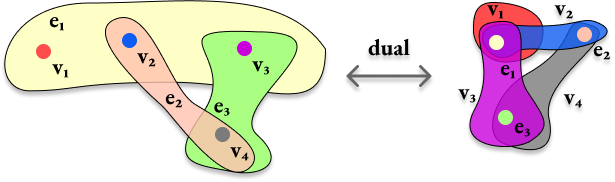
\includegraphics[width=\columnwidth]{duality}
 \captionsetup{belowskip=-14pt,aboveskip=3pt}
 \caption{Illustration of the dual of a hypergraph. 
 Left: a hypergraph with 4 nodes $v_1, v_2, v_3, v_4$ and 3 hyperedges $e_1=(v_1, v_2, v_3), e_2=(v_2, v_3), e_3=(v_3, v_4)$. 
 Right: the dual of the hypergraph, where the nodes and hyperedges interchanged.
 Nodes in the dual hypergraph are now $e_1, e_2, e_3$ and hyperedges are $v_1=(e_1), v_2=(e_1, e_2), v_3=(e_1, e_3), v_4=(e_2, e_3)$.
 }

\label{fig: duality}
\end{figure}

\subsubsection{Hierarchical Clustering}\label{sec: clustering}
Common clustering algorithms for graphs consider only graph connectivity.
However, for the best interpretability of the clustering result, the node embeddings must be also used in the clustering process.
This limits our choice of clustering algorithms to attributed node clustering algorithms.
Although there are existing approaches that can cluster attributed nodes on graphs such as EVA~\cite{citraro2020eva} and iLouvain~\cite{combe2015louvain}, they are not designed for hypergraphs.
In general, hypergraphs can be clustered in two different ways: 
(1) Directly operate on the hyperedges by generalizing the graph clustering algorithms.
For example, Kamiński et al.~\cite{kaminski2021hgraphcommunity} generalizes the modularity metric for graphs to hypergraphs; 
(2) First transform the hypergraph into a graph and then apply normal graph clustering algorithms~\cite{kumar2020new}.
Although the first approach is more intuitive, it is less scalable and hard to incorporate node attributes.
Thus, we have decided to design our clustering algorithm following the second approach.

Considering all the above, we implemented our hierarchical clustering algorithm by first transforming the hypergraph into a graph following the edge re-weighting process proposed by Kumar et al.~\cite{kumar2020new}.
Then an agglomerative clustering algorithm~\cite{steinbach2000doccluster} is applied on the re-weighted graph.
In agglomerative clustering, the key is to define node similarity and cluster similarity.
We can easily incorporate node attributes into the clustering process by defining the similarity between nodes and clusters as a weighted sum of attribute similarity $S_s$ and connectivity similarity $S_c$.
Since we're dealing with texts, we refer to the attribute similarity between nodes as semantic similarity. 

The semantic similarity $S_s(i, j)$ is the cosine similarity of the embeddings (dense vectors) of the two nodes, denoted as $vec_i$ and $vec_j$.
% For article nodes, the embeddings are generated using the article summaries.
% For participant nodes, the embeddings are generated using a description note of the participant.
% More details about the embeddings are explained in~\autoref{sec: embeddings}.
The connectivity similarity $S_c$ is the weighted Topological Overlap (wTO)~\cite{gysi2018wto},
which is a weighted generalization of the Overlap Coefficient~\cite{vijaymeena2016survey}, as shown in~\autoref{eq: connectivity_semantic_similarity}.
\begin{equation}\label{eq: connectivity_semantic_similarity}
    \mathbf{S_s}(i, j) = \frac{vec_i \cdot vec_j}{||vec_i|| \cdot ||vec_j||}, \quad
    \mathbf{S_c}(i, j) = \frac{\sum_{u=1}^N{w_{i,u}w_{u_j}} + w_{i,j}}{\min(k_i, k_j) + 1 - |w_{i,j}|}
\end{equation}
where $k_i = \sum_{j=1}^N |w_{i,j}|$ is the total weight of the edges connected to node $i$.
Finally, a weighting factor $\alpha$ is used to balance the two similarities, as shown in~\autoref{eq: similarity}.
\begin{equation}\label{eq: similarity}
    \mathbf{S} = \alpha \mathbf{S_s} + (1-\alpha) \mathbf{S_c}
\end{equation}
For the similarity between clusters, we used centroid similarity, i.e.\ the similarity between two clusters is the similarity between the centroids of the two clusters.
The algorithm takes a hypergraph $H=(V, E)$ and the embeddings of each node $Vec$ as input, and outputs a sequence of partitions $P=P_1, P_2, \dots P_k$.
Each partition corresponds to a level in the hierarchy, as shown in Algorithm 1.
\begin{algorithm}\label{alg: clustering}
    \caption{Agglomerative Clustering }\label{alg:cap}
    \hspace*{\algorithmicindent} \textbf{Input}: $H=(V, E)$, $Vec=\{vec_i |\, i \in V\}$ \\
    \hspace*{\algorithmicindent} \textbf{Output}: Sequence of partitions $\mathbf{P}=P_1, P_2, \dots P_k$ \\
    \begin{algorithmic}[1]
    \While{$|V| > 1$}
        \State$P_k = init\_partition(V)$ \Comment{Initialize each node as a cluster}
        \State$\mathbf{S_s} = cosine\_similarity(V\times V, Vec)$ 
        \State$\mathbf{S_c} = wTO(V\times V, E)$ \
        \For{$i \in V$}
            \State$j = most\_similar\_node(i, S_s, S_c)$ 
            \State$P_k = merge\_clusters(i, j)$ \Comment{Merge the two clusters}
        \EndFor
        \State$H^\prime=(V^\prime, E^\prime) = construct\_hypergraph(P_k)$ \Comment{clusters are the new nodes}
        \State$Vec^\prime = centroid\_similarity(V^\prime)$
        \State$V=V^\prime, E=E^\prime, Vec=Vec^\prime$ \Comment{Update for next iteration}
    \EndWhile
    \end{algorithmic}
\end{algorithm}


